\documentclass[tikz,border=5pt]{standalone}
\usepackage{newtxtext,newtxmath}
\usetikzlibrary{arrows.meta,calc,fit,positioning}

\definecolor{axisx}{HTML}{DCEBFA}
\definecolor{axisy}{HTML}{DDF3E4}
\definecolor{axisz}{HTML}{FCE8D5}
\definecolor{groupborder}{HTML}{7A8793}
\definecolor{labelgray}{HTML}{4A5560}

\begin{document}
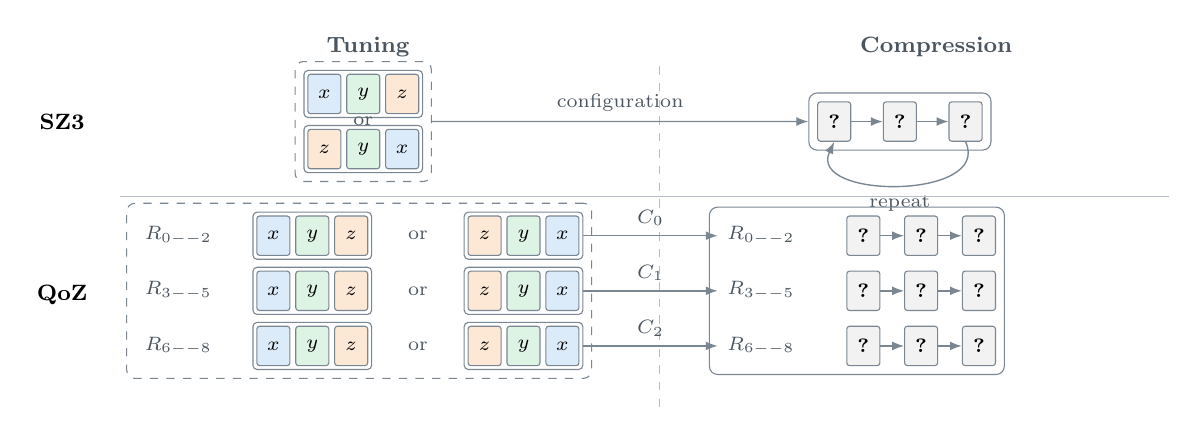
\begin{tikzpicture}[x=1.85cm,y=1cm,
axis/.style={draw=groupborder,rounded corners=1pt,minimum width=4.2mm,minimum height=5mm,inner sep=0pt,font=\scriptsize},
candidate/.style={draw=groupborder,rounded corners=1.5pt,inner sep=1.2pt},
tuningpanel/.style={draw=groupborder,dashed,rounded corners=3pt,inner sep=3pt},
compressionpanel/.style={draw=groupborder,rounded corners=3pt,inner sep=3pt},
roundlabel/.style={font=\scriptsize,text=labelgray,anchor=west},
note/.style={font=\scriptsize,text=labelgray},
flow/.style={-{Latex[length=1.5mm]},draw=groupborder,line width=.5pt},
stage/.style={font=\bfseries\footnotesize,text=labelgray}
]
\node[stage]at(2.35,3.05){Tuning};
\node[stage]at(6.25,3.05){Compression};
\draw[groupborder!55,dashed] (4.35,2.8)--(4.35,-1.55);

\node[font=\bfseries\footnotesize]at(.25,2.1){SZ3};
\node[axis,fill=axisx](sfx)at(2.05,2.45){$x$};
\node[axis,fill=axisy,right=.6mm of sfx](sfy){$y$};
\node[axis,fill=axisz,right=.6mm of sfy](sfz){$z$};
\node[candidate,fit=(sfx)(sfz)](sf){};
\node[axis,fill=axisz](srz)at(2.05,1.75){$z$};
\node[axis,fill=axisy,right=.6mm of srz](sry){$y$};
\node[axis,fill=axisx,right=.6mm of sry](srx){$x$};
\node[candidate,fit=(srz)(srx)](sr){};
\node[note]at($(sf.south)!.5!(sr.north)$){or};
\node[tuningpanel,fit=(sf)(sr)](stuning){};

\node[axis,fill=black!5,font=\bfseries\scriptsize](sq0)at(5.55,2.1){?};
\node[axis,fill=black!5,font=\bfseries\scriptsize,right=4mm of sq0](sq1){?};
\node[axis,fill=black!5,font=\bfseries\scriptsize,right=4mm of sq1](sq2){?};
\draw[flow](sq0.east)--(sq1.west);
\draw[flow](sq1.east)--(sq2.west);
\node[compressionpanel,fit=(sq0)(sq2)](scycle){};
\draw[flow](sq2.south)to[out=-65,in=-115,looseness=1.25]node[below,note]{repeat}(sq0.south);
\draw[flow](stuning.east)--node[above,note]{configuration}(scycle.west);

\draw[groupborder!55] (.65,1.15)--(7.85,1.15);

\node[font=\bfseries\footnotesize]at(.25,-.1){QoZ};
\node[roundlabel](tl0)at(.75,.65){$R_{0\text{--}2}$};
\node[axis,fill=axisx](t00)at(1.7,.65){$x$};
\node[axis,fill=axisy,right=.6mm of t00](t01){$y$};
\node[axis,fill=axisz,right=.6mm of t01](t02){$z$};
\node[candidate,fit=(t00)(t02)](tf0){};
\node[axis,fill=axisz](u00)at(3.15,.65){$z$};
\node[axis,fill=axisy,right=.6mm of u00](u01){$y$};
\node[axis,fill=axisx,right=.6mm of u01](u02){$x$};
\node[candidate,fit=(u00)(u02)](tr0){};
\node[note]at($(tf0.east)!.5!(tr0.west)$){or};

\node[roundlabel](tl1)at(.75,-.05){$R_{3\text{--}5}$};
\node[axis,fill=axisx](t10)at(1.7,-.05){$x$};
\node[axis,fill=axisy,right=.6mm of t10](t11){$y$};
\node[axis,fill=axisz,right=.6mm of t11](t12){$z$};
\node[candidate,fit=(t10)(t12)](tf1){};
\node[axis,fill=axisz](u10)at(3.15,-.05){$z$};
\node[axis,fill=axisy,right=.6mm of u10](u11){$y$};
\node[axis,fill=axisx,right=.6mm of u11](u12){$x$};
\node[candidate,fit=(u10)(u12)](tr1){};
\node[note]at($(tf1.east)!.5!(tr1.west)$){or};

\node[roundlabel](tl2)at(.75,-.75){$R_{6\text{--}8}$};
\node[axis,fill=axisx](t20)at(1.7,-.75){$x$};
\node[axis,fill=axisy,right=.6mm of t20](t21){$y$};
\node[axis,fill=axisz,right=.6mm of t21](t22){$z$};
\node[candidate,fit=(t20)(t22)](tf2){};
\node[axis,fill=axisz](u20)at(3.15,-.75){$z$};
\node[axis,fill=axisy,right=.6mm of u20](u21){$y$};
\node[axis,fill=axisx,right=.6mm of u21](u22){$x$};
\node[candidate,fit=(u20)(u22)](tr2){};
\node[note]at($(tf2.east)!.5!(tr2.west)$){or};
\node[tuningpanel,fit=(tl0)(tr0)(tl2)(tr2)](qtuning){};

\node[roundlabel](cl0)at(4.75,.65){$R_{0\text{--}2}$};
\node[axis,fill=black!5,font=\bfseries\scriptsize](q00)at(5.75,.65){?};
\node[axis,fill=black!5,font=\bfseries\scriptsize,right=3mm of q00](q01){?};
\node[axis,fill=black!5,font=\bfseries\scriptsize,right=3mm of q01](q02){?};
\draw[flow](q00.east)--(q01.west);
\draw[flow](q01.east)--(q02.west);

\node[roundlabel](cl1)at(4.75,-.05){$R_{3\text{--}5}$};
\node[axis,fill=black!5,font=\bfseries\scriptsize](q10)at(5.75,-.05){?};
\node[axis,fill=black!5,font=\bfseries\scriptsize,right=3mm of q10](q11){?};
\node[axis,fill=black!5,font=\bfseries\scriptsize,right=3mm of q11](q12){?};
\draw[flow](q10.east)--(q11.west);
\draw[flow](q11.east)--(q12.west);

\node[roundlabel](cl2)at(4.75,-.75){$R_{6\text{--}8}$};
\node[axis,fill=black!5,font=\bfseries\scriptsize](q20)at(5.75,-.75){?};
\node[axis,fill=black!5,font=\bfseries\scriptsize,right=3mm of q20](q21){?};
\node[axis,fill=black!5,font=\bfseries\scriptsize,right=3mm of q21](q22){?};
\draw[flow](q20.east)--(q21.west);
\draw[flow](q21.east)--(q22.west);
\node[compressionpanel,fit=(cl0)(q02)(cl2)(q22)](qcompression){};

\draw[flow](tr0.east)--node[above,note]{$C_0$}(cl0.west);
\draw[flow](tr1.east)--node[above,note]{$C_1$}(cl1.west);
\draw[flow](tr2.east)--node[above,note]{$C_2$}(cl2.west);
\end{tikzpicture}
\end{document}
